\documentclass[border=0.2cm]{standalone}

\usepackage{tikz}
\usetikzlibrary{automata, positioning}

\begin{document}

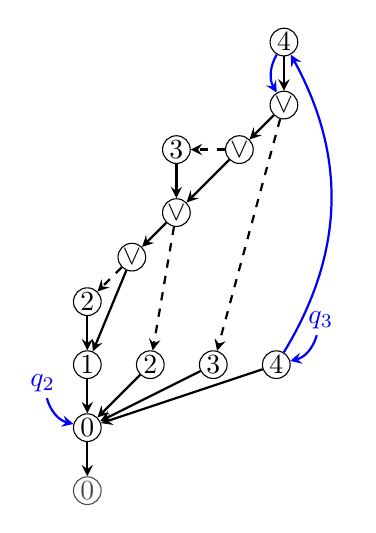
\begin{tikzpicture}[node distance = 0.8cm,
  on grid,
  auto,
]

\tikzstyle{initial}= [black!70]
\tikzstyle{every state}=[inner sep=0pt, minimum size=10pt]

%%%%%%%%%%%%%%%%%%%%%%%%%%%%%%%% Nodes

\node (0') [state, initial] {$0$};
\node (0)  [state, above = of 0'] {$0$};
\node (1)  [state, above = of 0] {$1$};
\node (2l) [state, above = of 1] {$2$};
\node (2r) [state, above right = of 0, right = of 1] {$2$};
\node (v1) [state, above right = of 2l] {$\lor$};
\node (v2) [state, above right = of v1] {$\lor$};
\node (3l) [state, above = of v2] {$3$};
\node (3r) [state, right = of 2r] {$3$};
\node (v3) [state, above right = of v2, right = of 3l] {$\lor$};
\node (v4) [state, above right = of v3] {$\lor$};
\node (4l) [state, above = of v4] {$4$};
\node (4r) [state, right = of 3r] {$4$};

\path [-stealth, thick]
    (0) edge node {} (0')
    (1) edge node {} (0)
    (2l) edge node {} (1)
    (2r) edge node {} (0)
    (v1) edge [dashed] node {} (2l)
    (v1) edge node {} (1)
    (v2) edge [dashed] node {} (2r)
    (v2) edge node {} (v1)
    (3l) edge node {} (v2)
    (3r) edge node {} (0)
    (v3) edge [dashed] node {} (3l)
    (v3) edge node {} (v2)
    (v4) edge [dashed] node {} (3r)
    (v4) edge node {} (v3)
    (4r) edge node {} (0)
    (4l) edge node {} (v4)
    ;

%%%%%%%%%%%%%%%%%%%%%%%%%%%%%%%% States/ul

\node (q2)  [state, above left= of 0, draw=none]   [color=blue] {$q_{2}$};
\node (q3)  [state, above right = of 4r, draw=none] [color=blue] {$q_{3}$};

\path [-stealth, thick, color=blue]
    (q2) edge [bend right] node {} (0)
    (q3) edge [bend left] node {} (4r)
    (4r) edge [bend right] node {} (4l)
    (4l) edge [bend right] node {} (v4)
    ;

\end{tikzpicture}
\end{document}
